\documentclass[14pt]{extbook}
\usepackage{multicol, enumerate, enumitem, hyperref, color, soul, setspace, parskip, fancyhdr} %General Packages
\usepackage{amssymb, amsthm, amsmath, latexsym, units, mathtools} %Math Packages
\everymath{\displaystyle} %All math in Display Style
% Packages with additional options
\usepackage[headsep=0.5cm,headheight=12pt, left=1 in,right= 1 in,top= 1 in,bottom= 1 in]{geometry}
\usepackage[usenames,dvipsnames]{xcolor}
\usepackage{dashrule}  % Package to use the command below to create lines between items
\newcommand{\litem}[1]{\item#1\hspace*{-1cm}\rule{\textwidth}{0.4pt}}
\pagestyle{fancy}
\lhead{Progress Quiz 7}
\chead{}
\rhead{Version C}
\lfoot{3510-5252}
\cfoot{}
\rfoot{Summer C 2021}
\begin{document}

\begin{enumerate}
\litem{
Determine the domain of the function below.\[ f(x) = \frac{4}{18x^{2} +36 x + 16} \]\begin{enumerate}[label=\Alph*.]
\item \( \text{All Real numbers except } x = a, \text{ where } a \in [-25.3, -23] \)
\item \( \text{All Real numbers except } x = a, \text{ where } a \in [-2.2, -0.9] \)
\item \( \text{All Real numbers.} \)
\item \( \text{All Real numbers except } x = a \text{ and } x = b, \text{ where } a \in [-25.3, -23] \text{ and } b \in [-13.3, -11.7] \)
\item \( \text{All Real numbers except } x = a \text{ and } x = b, \text{ where } a \in [-2.2, -0.9] \text{ and } b \in [-1.1, 0.1] \)

\end{enumerate} }
\litem{
Choose the graph of the equation below.\[ f(x) = \frac{1}{(x - 3)^2} + 3 \]\begin{enumerate}[label=\Alph*.]
\begin{multicols}{2}\item 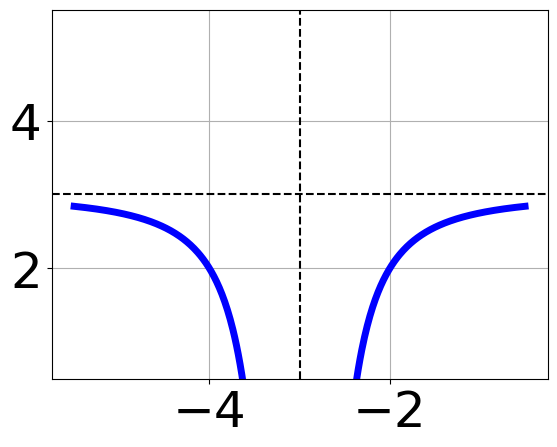
\includegraphics[width = 0.3\textwidth]{../Figures/rationalEquationToGraphAC.png}\item 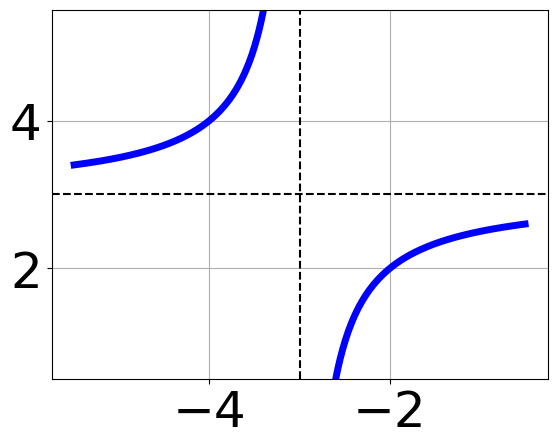
\includegraphics[width = 0.3\textwidth]{../Figures/rationalEquationToGraphBC.png}\item 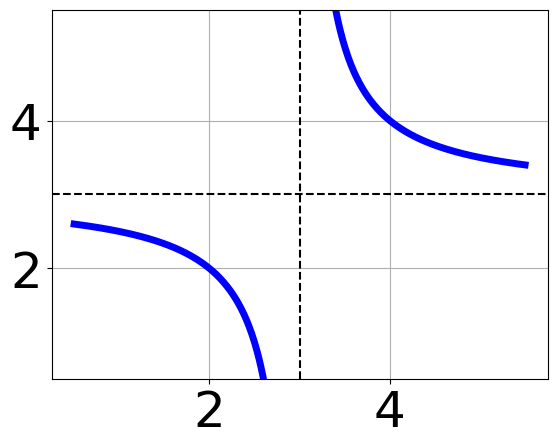
\includegraphics[width = 0.3\textwidth]{../Figures/rationalEquationToGraphCC.png}\item 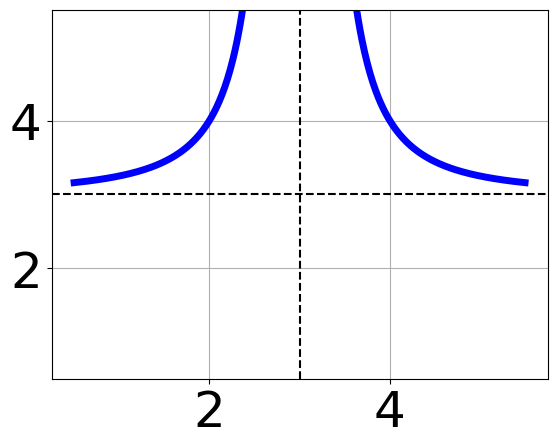
\includegraphics[width = 0.3\textwidth]{../Figures/rationalEquationToGraphDC.png}\end{multicols}\item None of the above.
\end{enumerate} }
\litem{
Choose the graph of the equation below.\[ f(x) = \frac{1}{x + 2} - 2 \]\begin{enumerate}[label=\Alph*.]
\begin{multicols}{2}\item 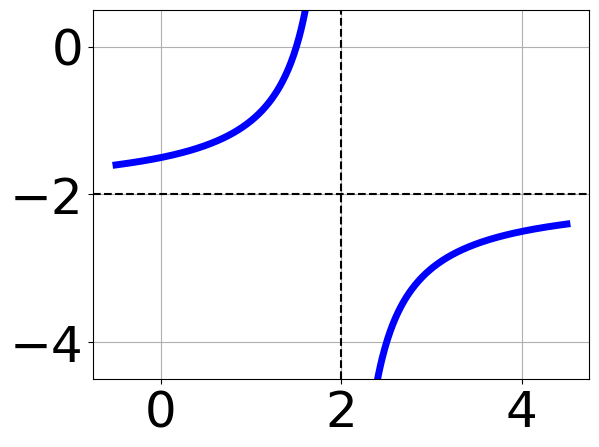
\includegraphics[width = 0.3\textwidth]{../Figures/rationalEquationToGraphCopyAC.png}\item 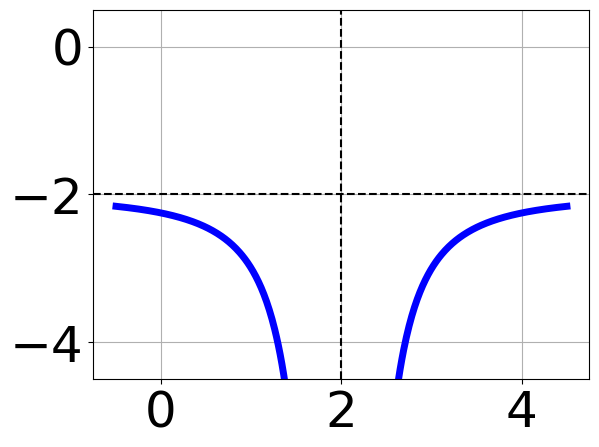
\includegraphics[width = 0.3\textwidth]{../Figures/rationalEquationToGraphCopyBC.png}\item 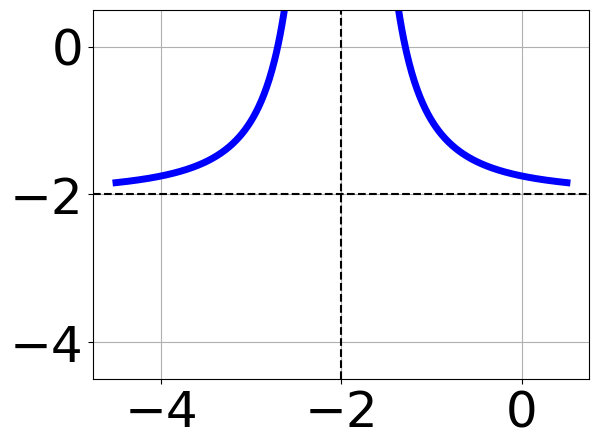
\includegraphics[width = 0.3\textwidth]{../Figures/rationalEquationToGraphCopyCC.png}\item 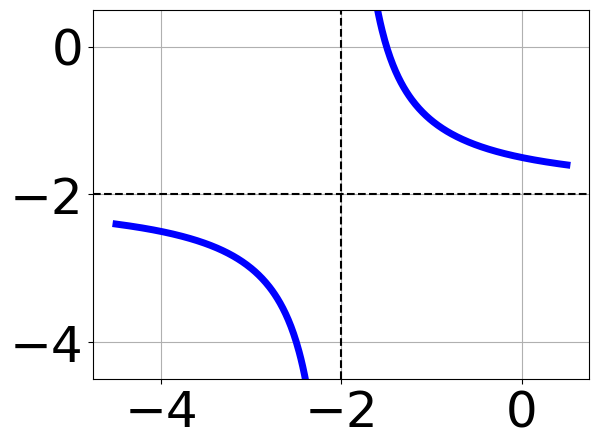
\includegraphics[width = 0.3\textwidth]{../Figures/rationalEquationToGraphCopyDC.png}\end{multicols}\item None of the above.
\end{enumerate} }
\litem{
Choose the equation of the function graphed below.
\begin{center}
    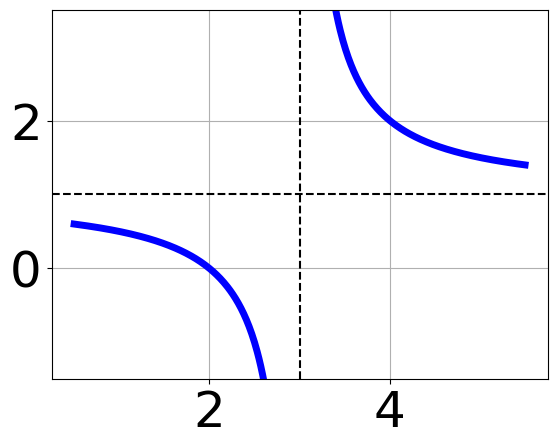
\includegraphics[width=0.5\textwidth]{../Figures/rationalGraphToEquationC.png}
\end{center}
\begin{enumerate}[label=\Alph*.]
\item \( f(x) = \frac{-1}{x + 3} + 1 \)
\item \( f(x) = \frac{-1}{(x + 3)^2} + 1 \)
\item \( f(x) = \frac{1}{x - 3} + 1 \)
\item \( f(x) = \frac{1}{(x - 3)^2} + 1 \)
\item \( \text{None of the above} \)

\end{enumerate} }
\litem{
Choose the equation of the function graphed below.
\begin{center}
    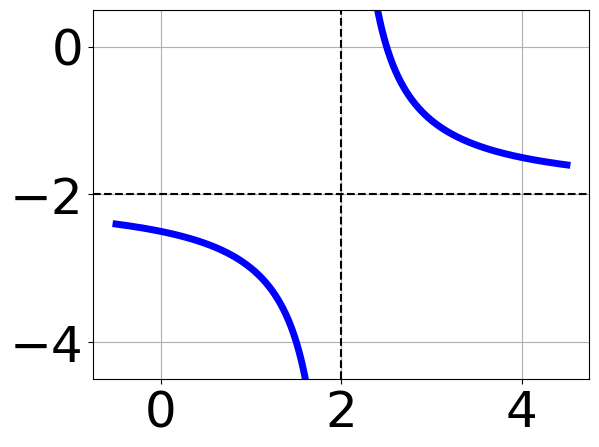
\includegraphics[width=0.5\textwidth]{../Figures/rationalGraphToEquationCopyC.png}
\end{center}
\begin{enumerate}[label=\Alph*.]
\item \( f(x) = \frac{1}{x + 2} - 5 \)
\item \( f(x) = \frac{-1}{x - 2} - 5 \)
\item \( f(x) = \frac{1}{(x + 2)^2} - 5 \)
\item \( f(x) = \frac{-1}{(x - 2)^2} - 5 \)
\item \( \text{None of the above} \)

\end{enumerate} }
\litem{
Solve the rational equation below. Then, choose the interval(s) that the solution(s) belongs to.\[ \frac{-10}{40x + 20} + 1 = \frac{-10}{40x + 20} \]\begin{enumerate}[label=\Alph*.]
\item \( x \in [0,1.4] \)
\item \( x_1 \in [-0.9, -0.3] \text{ and } x_2 \in [-1.8,0.3] \)
\item \( x_1 \in [-0.9, -0.3] \text{ and } x_2 \in [-0.4,1.5] \)
\item \( x \in [-0.5,1.5] \)
\item \( \text{All solutions lead to invalid or complex values in the equation.} \)

\end{enumerate} }
\litem{
Solve the rational equation below. Then, choose the interval(s) that the solution(s) belongs to.\[ \frac{6}{-2x -9} + -3 = \frac{-4}{18x + 81} \]\begin{enumerate}[label=\Alph*.]
\item \( x \in [3.1,3.8] \)
\item \( x \in [-5.43,-4.43] \)
\item \( \text{All solutions lead to invalid or complex values in the equation.} \)
\item \( x_1 \in [-6.7, -5.6] \text{ and } x_2 \in [-5.43,-3.43] \)
\item \( x_1 \in [-5.5, -5.2] \text{ and } x_2 \in [2.57,4.57] \)

\end{enumerate} }
\litem{
Determine the domain of the function below.\[ f(x) = \frac{6}{24x^{2} -38 x + 15} \]\begin{enumerate}[label=\Alph*.]
\item \( \text{All Real numbers except } x = a, \text{ where } a \in [0.71, 0.77] \)
\item \( \text{All Real numbers.} \)
\item \( \text{All Real numbers except } x = a \text{ and } x = b, \text{ where } a \in [0.71, 0.77] \text{ and } b \in [0.82, 0.85] \)
\item \( \text{All Real numbers except } x = a, \text{ where } a \in [11.91, 12.1] \)
\item \( \text{All Real numbers except } x = a \text{ and } x = b, \text{ where } a \in [11.91, 12.1] \text{ and } b \in [29.9, 30.18] \)

\end{enumerate} }
\litem{
Solve the rational equation below. Then, choose the interval(s) that the solution(s) belongs to.\[ \frac{-2x}{2x + 2} + \frac{-4x^{2}}{-12x^{2} -18 x -6} = \frac{-7}{-6x -3} \]\begin{enumerate}[label=\Alph*.]
\item \( x_1 \in [-1.47, -1.27] \text{ and } x_2 \in [-0.26,0.74] \)
\item \( x \in [-0.58,-0.31] \)
\item \( \text{All solutions lead to invalid or complex values in the equation.} \)
\item \( x_1 \in [-1.18, -0.67] \text{ and } x_2 \in [-1.64,-0.49] \)
\item \( x \in [-1.18,-0.67] \)

\end{enumerate} }
\litem{
Solve the rational equation below. Then, choose the interval(s) that the solution(s) belongs to.\[ \frac{-3x}{-6x + 5} + \frac{-2x^{2}}{-12x^{2} +52 x -35} = \frac{-4}{2x -7} \]\begin{enumerate}[label=\Alph*.]
\item \( x \in [3.15,4.34] \)
\item \( x \in [-3.35,-0.26] \)
\item \( x_1 \in [0.39, 3.08] \text{ and } x_2 \in [-1.17,7.83] \)
\item \( x_1 \in [0.39, 3.08] \text{ and } x_2 \in [-2.78,-0.78] \)
\item \( \text{All solutions lead to invalid or complex values in the equation.} \)

\end{enumerate} }
\end{enumerate}

\end{document}